\documentclass{article}
\usepackage{graphicx}
\begin{document}
Graphics inline 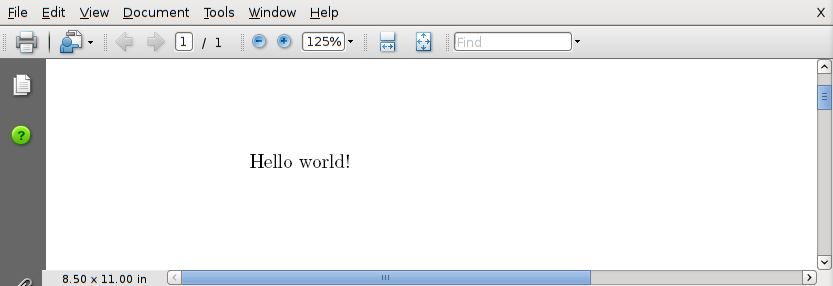
\includegraphics{graphics/raster} in a line of text, then a
scaled one 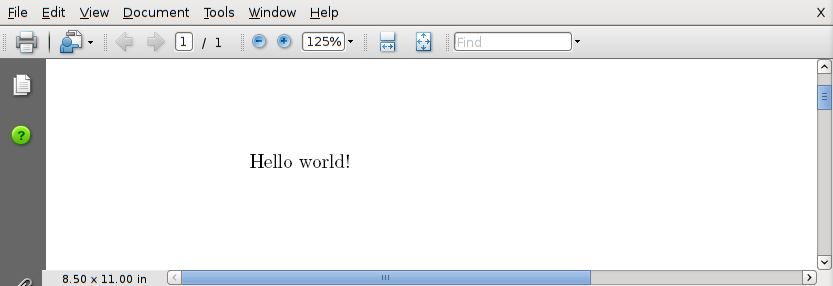
\includegraphics[scale=.35]{graphics/raster.png} and text after it.


\includegraphics[width=3cm]{graphics/vector}

\includegraphics[height=1in]{graphics/vector.pdf}

\includegraphics[width=0.5\textwidth,height=2cm]{graphics/vector}

\includegraphics[width=0.5\textwidth,height=2cm,keepaspectratio]{graphics/vector}

\begin{figure}[h]
\centering
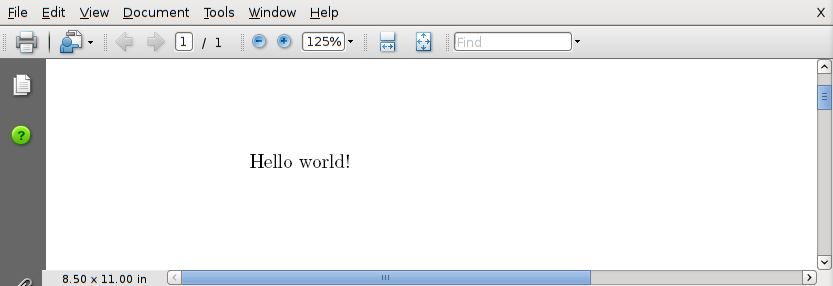
\includegraphics[width=.4\linewidth]{graphics/raster}
\caption{The same raster again, at a width.}
\end{figure}

A paragraph after the figure, and 
\includegraphics[height=2ex]{graphics/vector} once more.
\end{document}
